Pac-Man is a maze-chase video game developed in 1980s. 
The player controls the character ``Pac-Man'' to eat dots in a maze while
avoiding enemy characters ``ghosts.'' 
All characters may move in four directions: up, down, left, right.
The game ends in two conditions:
\begin{itemize}
\item Pac-Man eats all dots in the maze. In this case, the player wins.
\item Any ghost catches Pac-Man. In this case, the player loses.
\end{itemize}

\begin{figure}[h]
\center
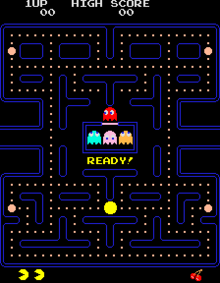
\includegraphics[width=0.25\textwidth]{image/pacman.png}
\caption{Pac-Man gameplay (image from Wikipedia)}
\end{figure}

Adam is learning how to create games with modern programming tools.
To practice the skills, he tries to make an imitation of the Pac-Man 
game with some modification.
In this game, the playable character is a ``ghost,'' 
and the enemy character is ``Pac-Man.'' 
Since he changes the roles of the ghost and Pac-Man, 
he also changes the ending conditions of the game.
\begin{itemize}
\item Pac-Man eats all dots in the maze. In this case, the player loses.
\item The ghost controlled by the player catches Pac-Man. In this case, the player wins.
\end{itemize}

Adam has almost developed the first full functioning version of his game.
He creates a simple stage for testing.
The maze of the stage is based on 10-by-10 grid, and each grid cell contains 
exact one dot.
Inside the grid, there are no walls or obstacles.
 

To prepare the movement of Pac-Man, Adam uses crowd sourcing.


